\documentclass[a4paper,10pt,twocolumn]{ltjsarticle}
\usepackage[haranoaji]{luatexja-preset}
\usepackage[top=18mm,bottom=20mm,left=17mm,right=17mm,columnsep=8mm]{geometry}
\usepackage{graphicx,booktabs,array,caption,enumitem,xcolor,tikz}
\usetikzlibrary{shapes.geometric}
\setlength{\parindent}{1\zw}
\renewcommand{\baselinestretch}{1.0}
\setlength{\parskip}{0pt}
\renewcommand{\thesection}{\arabic{section}.}
\renewcommand{\thesubsection}{\arabic{section}.\arabic{subsection}.}
\makeatletter
\renewcommand{\section}{\@startsection{section}{1}{\z@}{1.1\Cvs \@plus.4\Cdp \@minus.2\Cdp}{.5\Cvs \@plus.2\Cdp}{\normalfont\gtfamily\bfseries\large}}
\renewcommand{\subsection}{\@startsection{subsection}{2}{\z@}{.8\Cvs \@plus.3\Cdp \@minus.2\Cdp}{.3\Cvs \@plus.1\Cdp}{\normalfont\gtfamily\bfseries\normalsize}}
\makeatother
\captionsetup{font={small,sf},labelsep=space,justification=raggedright,singlelinecheck=false,skip=3pt}
\captionsetup[table]{position=top}
\setlist[itemize]{leftmargin=1.2\zw,itemsep=0pt,topsep=2pt,parsep=0pt}
\setlength{\textfloatsep}{8pt plus 2pt minus 2pt}
\setlength{\floatsep}{8pt plus 2pt minus 2pt}
\setlength{\intextsep}{8pt plus 2pt minus 2pt}
\pagestyle{plain}
\raggedbottom
\begin{document}
\twocolumn[{
\noindent\fbox{\gtfamily\small\ 生成AI論文\ }\par\medskip
\begin{center}
{\gtfamily\bfseries\LARGE 算数・数学を「とても好き」と答える子の割合と国・地域の平均得点：TIMSS 2023の公表値による国際比較$^{\dagger}$}\par\medskip
{\gtfamily\bfseries\large 小4・中2の「好き」「自信」「価値」と得点の関連を国・地域別に整理する}\par\medskip
{\normalsize EduData調査研究グループ$^{*1}$・教育データサイエンス解析班$^{*2}$}\par
{\small オープン教育統計推進プロジェクト$^{*1}$・初等中等STEM教育データ基盤ユニット$^{*2}$}
\end{center}\smallskip
\noindent\begin{minipage}{\textwidth}\small 本研究は，TIMSS 2023の国・地域別公表値（小4は58，中2は43の国・地域）を用い，算数・数学を「とても好き」「とても自信あり」「とても価値あり」と答えた児童生徒の割合が，国・地域の平均得点とどう関連するかを整理した．その結果，「とても好き」の割合は平均得点と負に関連し（小4 \textit{r}=−.65，中2 \textit{r}=−.67），中2の「とても価値あり」も同様であった（\textit{r}=−.74）．一方，「とても自信あり」の割合は平均得点とほとんど関連しなかった（小4 \textit{r}=−.12，中2 \textit{r}=.12）．中2では「好き」と「価値」の割合が非常に強く連動した（\textit{r}=.93）．日本は平均得点が小4で5位，中2で4位であり，「とても好き」は小4で22\%，中2で10\%，中2の「自信なし」は74\%であった．これらは国・地域を単位とした集計値の関連であり，個々の児童生徒の因果や理由を示すものではない．回答の仕方の文化差や，国内の集団ごとの比較にもとづく解釈の可能性を考察した．\par\smallskip
\noindent{\gtfamily キーワード：}TIMSS 2023，算数・数学教育，情意，国際比較，生態学的誤謬\end{minipage}\medskip
}]
\let\thefootnote\relax
\footnotetext{\footnotesize 2026年10月執筆\\ $^{\dagger}$Liking, Confidence and Valuing of Mathematics and National Achievement in TIMSS 2023: A Country-Level Comparison\\ $^{*1}$ Open Education Data Project, Tokyo, Japan\quad $^{*2}$ Educational Data Science Unit, Tokyo, Japan}
\section{はじめに}
\subsection{研究の背景}
算数・数学を好きだと感じること，自分にできるという自信，そして学ぶ価値の認識は，学習への動機づけの中心にあると考えられてきた．Wigfield and Eccles (2000)の期待価値理論は，成功への期待と課題の価値が課題の選択や遂行を規定すると述べ，Bandura (1997)は自己効力感が行動の遂行を左右すると論じた．Pekrun (2006)の統制-価値理論は，楽しさなどの学業にかかわる感情が，状況への統制の感覚と価値の評価から生じると整理している．これらはいずれも，個人の内側の関係を説明する理論である．

国際比較では，個人の内側の関係と，国・地域を単位とした関係とが一致するとは限らない．集団レベルの相関から個人の関係を読み取る誤りは，Robinson (1950)が生態学的誤謬として指摘した．TIMSSの複数回のデータを分析したShen and Tam (2008)は，得点と自己認識の関連が国レベルで逆説的に現れることを報告している．またLee and Stankov (2018)は，TIMSSとPISAを用いて，個人レベルでは自信などの自己認識が数学の得点を最もよく予測する要因であると整理した．

IEA (2024)が公表したTIMSS 2023の結果では，日本は小4・中2とも得点が上位にある一方，「好き」「自信」の肯定的な回答の割合は高くない．この組み合わせが日本に特有なのか，国際的な傾向なのかは，公表値を並べてみないと分からない．
\subsection{リサーチクエスチョン}
本研究の目的は，TIMSS 2023の国・地域別公表値を用いて，算数・数学に対する情意（好き・自信・価値）の肯定的な回答の割合と，国・地域の平均得点との関連を記述することである．次の2つの研究課題を置く．
\begin{itemize}
\item RQ1：「とても好き」の割合が高い国・地域ほど，平均得点は高いか．小4と中2で傾向は同じか．
\item RQ2：「自信」「価値」の割合は，平均得点や「好き」の割合とどう関連するか．日本はこの中でどこに位置するか．
\end{itemize}
\section{調査対象および分析方法}
TIMSS 2023の公表表から，国・地域ごとの値を集めた．小4は58，中2は43の国・地域のデータがあり，両学年に参加した国・地域は37，全体では64の国・地域である．小4と中2は別の集団なので，分析は学年ごとに別々に行い，学年を混ぜていない．児童生徒の質問紙への回答から作られた尺度のうち，「とても好き」「とても自信あり」「とても価値あり」（価値は中2のみ）の割合（\%）と，国・地域の平均得点を用いた．また，「好き層と好きでない層」「自信あり層と自信なし層」の間の平均得点の差（点）も用いた．

分析単位は国・地域で，各国・地域を同じ重みで扱った．関連の強さはピアソンの積率相関係数 \textit{r} で示し，あわせて \textit{p} 値とJZSベイズファクター（\textit{BF}\textsubscript{10}）を算出した．\textit{BF}\textsubscript{10}が3を超えれば関連を支持する証拠，1/3を下回れば関連がないことを支持する証拠とみなした．外れ値の影響を見るため，スピアマンの順位相関係数 \textit{ρ} と，\textit{r} の95\%信頼区間（フィッシャーのz変換）も示す．報告する指標のペアは研究課題にもとづいて選んだものであり，全ペアを探索した結果ではない．標本は国・地域ごとの抽出調査であり，ここで使った値は公表された集計値だけである．個票は用いていない．また，平均得点の低い3か国・地域を除いた場合も計算した．
\begin{table*}[!t]
\caption{主要指標の基本記述統計量}
\centering\small
\begin{tabular}{>{\raggedright\arraybackslash}p{9.2cm}rrrrrr}
\toprule
指標 & \textit{K} & 平均 & \textit{SD} & 中央値 & 最小 & 最大 \\
\midrule
小4・とても好き(\%) & 58 & 44.3 & 16.4 & 40.0 & 21.0 & 80.0 \\
小4・好きでない(\%) & 58 & 23.9 & 11.7 & 25.0 & 5.0 & 48.0 \\
小4・好き層と好きでない層の得点差 & 58 & 31.8 & 11.9 & 29.5 & 9.0 & 57.0 \\
小4・とても自信あり(\%) & 58 & 27.2 & 6.2 & 28.0 & 14.0 & 41.0 \\
小4・自信なし(\%) & 58 & 31.3 & 5.9 & 31.0 & 19.0 & 45.0 \\
小4・自信あり層と自信なし層の得点差 & 58 & 87.8 & 15.4 & 87.0 & 50.0 & 126.0 \\
小4・平均得点 & 58 & 503.2 & 56.0 & 514.5 & 362.0 & 615.0 \\
中2・とても好き(\%) & 43 & 21.3 & 12.3 & 18.0 & 7.0 & 56.0 \\
中2・好きでない(\%) & 43 & 46.3 & 15.1 & 49.0 & 11.0 & 69.0 \\
中2・好き層と好きでない層の得点差 & 43 & 49.5 & 22.2 & 50.0 & -2.0 & 89.0 \\
中2・とても自信あり(\%) & 43 & 12.9 & 3.5 & 13.0 & 4.0 & 20.0 \\
中2・自信なし(\%) & 43 & 55.4 & 6.9 & 54.0 & 43.0 & 74.0 \\
中2・自信あり層と自信なし層の得点差 & 43 & 109.1 & 20.1 & 111.0 & 50.0 & 167.0 \\
中2・とても価値ありと考える(\%) & 43 & 34.4 & 14.7 & 31.0 & 12.0 & 71.0 \\
中2・価値を感じない(\%) & 43 & 24.3 & 9.2 & 25.0 & 7.0 & 45.0 \\
中2・価値あり層と価値なし層の得点差 & 43 & 39.8 & 18.2 & 41.0 & -8.0 & 84.0 \\
中2・平均得点 & 43 & 473.5 & 70.6 & 488.0 & 263.0 & 605.0 \\
\bottomrule
\end{tabular}
\par\smallskip{\footnotesize 注）単位は\%，\textit{K}は観測数（国・地域・区分）．}
\end{table*}
\begin{table*}[!t]
\caption{主要指標間のピアソンの相関係数と，ベイズファクター}
\centering\small
\begin{tabular}{>{\raggedright\arraybackslash}p{6.4cm}>{\raggedright\arraybackslash}p{6.4cm}rrr}
\toprule
指標 \textit{X} & 指標 \textit{Y} & \textit{r} & \textit{p} & \textit{BF}\textsubscript{10} \\
\midrule
中2・とても好き(\%) & 中2・平均得点 & −.67 & < .001 & >1000 \\
小4・とても好き(\%) & 小4・好きでない(\%) & −.97 & < .001 & >1000 \\
小4・とても好き(\%) & 小4・好き層と好きでない層の得点差 & .27 & = .040 & 0.84 \\
小4・とても好き(\%) & 小4・とても自信あり(\%) & .45 & < .001 & 61.78 \\
小4・とても好き(\%) & 小4・自信なし(\%) & −.36 & = .005 & 5.18 \\
\bottomrule
\end{tabular}
\par\smallskip{\footnotesize 注）\textit{BF}\textsubscript{10}はJZSベイズファクター（3を超えれば関連を支持，1/3を下回れば関連がないことを支持）．全ペアの探索の一部を載せた．}
\end{table*}
\section{結果}
RQ1について，「とても好き」の割合と平均得点の間には，小4で中程度の負の相関（\textit{r}=−.65，95\%CI [−.78, −.47]，\textit{ρ}=−.75，\textit{n}=58，\textit{p}<.001，\textit{BF}\textsubscript{10}>1000），中2でも同程度の負の相関（\textit{r}=−.67，95\%CI [−.81, −.47]，\textit{ρ}=−.70，\textit{n}=43，\textit{p}<.001，\textit{BF}\textsubscript{10}>1000）が見られた．平均得点の低い3か国・地域を除いても，関連は変わらなかった（小4 \textit{r}=−.65，中2 \textit{r}=−.61）．すなわち，「とても好き」の割合が高い国・地域ほど，平均得点が低い傾向があった．得点の上位は，小4がシンガポール（615点，「とても好き」33\%），台湾（607点，22\%），香港（594点，37\%），韓国（594点，22\%），日本（591点，22\%）であり，中2はシンガポール（605点，24\%），台湾（602点，12\%），韓国（596点，12\%），日本（595点，10\%）であった．「とても好き」の割合が最も高いのは，小4・中2ともウズベキスタン（80\%，56\%）であった．

RQ2について，「とても自信あり」の割合と平均得点との関連は，小4で \textit{r}=−.12（95\%CI [−.37, .14]，\textit{p}=.37，\textit{BF}\textsubscript{10}=0.15），中2で \textit{r}=.12（95\%CI [−.19, .41]，\textit{p}=.44，\textit{BF}\textsubscript{10}=0.16）と，ほとんど見られなかった．一方，中2の「とても価値あり」の割合は平均得点と強い負の相関を示し（\textit{r}=−.74，95\%CI [−.85, −.56]，\textit{p}<.001，\textit{BF}\textsubscript{10}>1000），「とても好き」の割合とは非常に強い正の相関を示した（\textit{r}=.93，95\%CI [.87, .96]，\textit{p}<.001，\textit{BF}\textsubscript{10}>1000）．小4では「とても好き」と「とても自信あり」の割合が中程度に連動した（\textit{r}=.45，\textit{p}<.001，\textit{BF}\textsubscript{10}=61.78）が，中2では連動しなかった（\textit{r}=.09，\textit{p}=.57）．なお，小4の「とても好き」の割合と「好き層と好きでない層の得点差」の相関は弱く（\textit{r}=.27，\textit{p}=.040，\textit{BF}\textsubscript{10}=0.84），関連を支持する証拠は十分でなかった．

日本は，小4で「とても好き」22\%（最も低いのは21\%のポーランドで，台湾・韓国も22\%），「とても自信あり」14\%（平均27.2\%），「自信なし」45\%（平均31.3\%）であった．中2では「とても好き」10\%，「とても自信あり」4\%（平均12.9\%），「とても価値あり」13\%（平均34.4\%），「自信なし」74\%（平均55.3\%）であった．また，両学年に参加した37の国・地域では，「とても好き」の割合の平均は小4で45.5\%，中2で20.7\%であり，すべての国・地域で小4のほうが高かった．
\begin{figure}[t]\centering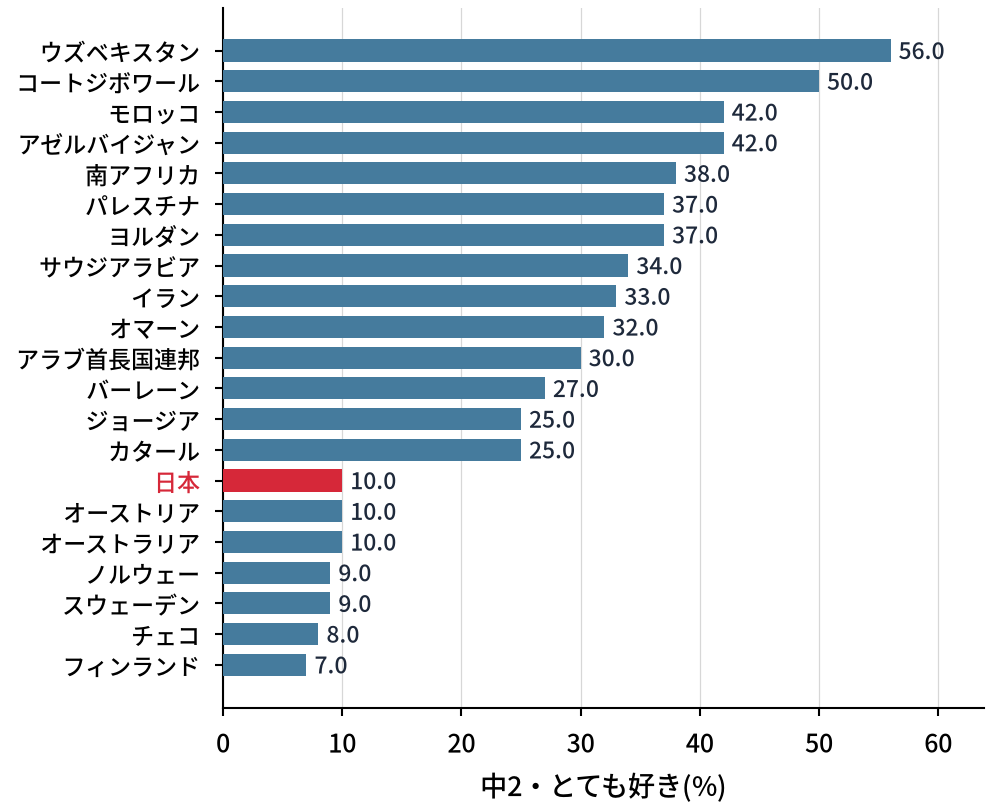
\includegraphics[width=\columnwidth]{chart_timss2023_student_attitudes.png}\caption{中2・とても好き(\%)の値の比較（上位・下位と日本を抜粋）．赤が日本}\end{figure}
\begin{figure}[t]\centering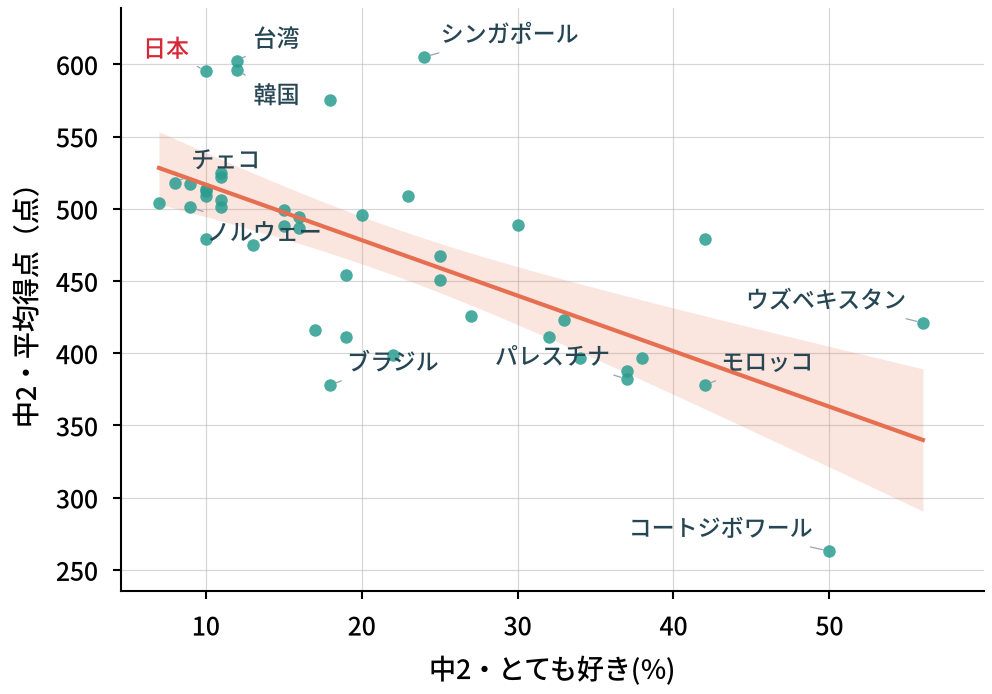
\includegraphics[width=\columnwidth]{chart_secondary_timss2023_student_attitudes.png}\caption{中2・とても好き(\%)と中2・平均得点の関連（回帰直線と，その平均の95\%信頼区間の帯，n=43）}\end{figure}
\section{考察}
RQ1とRQ2の結果をまとめると，国・地域を単位とした場合，「好き」や「価値」の肯定的な回答の割合が高い国ほど平均得点が低く，「自信」の割合は得点とほとんど関連しなかった．期待価値理論（Wigfield and Eccles，2000）は，個人の内側で価値と期待が動機づけを高めることを述べるもので，この結果はその理論と矛盾するとは言えない．個人レベルと国レベルの関連が食い違うことは，Robinson (1950)の生態学的誤謬やShen and Tam (2008)の報告と整合する．実際，Lee and Stankov (2018)は，個人レベルでは自信が数学の得点の主要な予測要因であると整理しており，本研究でも，国・地域のなかでは自信あり層と自信なし層の得点差が中2で平均109点に達する（トルコは167点）一方，国・地域の間では「自信」の割合が得点と関連しなかった．

この国レベルの関連の理由は，本研究のデータでは検証できない．可能性として，次の2つを挙げる．第一に，回答の仕方の違いである．Chen et al. (1995)は，日本と台湾の高校生が北米の高校生より尺度の中間を選びやすく，北米は両端を選びやすいことを示した．「とても好き」のような最も肯定的な選択肢の割合は，この影響を受けうる．ただし同研究では，この差は小さく，平均値の国際比較を大きく変えなかったとも報告されており，これだけで今回の関連を説明できるとは考えにくい．第二に，比較の基準の違いである．Marsh and Hau (2003)は，26か国の分析で，同程度の学力でも得点の高い学校に所属する生徒ほど学業的自己概念が低いことを示した．得点の高い国・地域でも，生徒が周囲との比較で自分を低く評価している可能性があるが，これは仮説にとどまる．また，中2の「好き」と「価値」の割合は強く連動し（\textit{r}=.93），どちらも得点と負に関連したが，この2つは別々の証拠ではなく，共通の要因（例えば回答の仕方）を反映した同じ現象である可能性がある．

日本は得点が上位でありながら，中2の「自信なし」が74\%と高い．この数字を，授業のあり方や教育制度の帰結と読むことはできない．一方で，国内では自信の有無による得点差が大きいことから，学級のなかで自信を育てる手立ては，意味のある課題として検討できる．本研究の限界は，(1)国・地域の集計値のみを用いており個人の因果を特定できないこと，(2)質問紙への自己報告であり回答の仕方の影響を受けうること，(3)小4と中2は別の集団であり，学年間の差を同じ子どもの変化と解釈できないこと，(4)家庭の経済状況や学校制度などを統制していないこと，である．今後は，個票を用いた個人レベルの分析と，回答の仕方を考慮した分析が必要である．
\section*{参考文献}
\begingroup\scriptsize\raggedright\interlinepenalty=10000 
\begin{list}{}{\setlength{\leftmargin}{1.5\zw}\setlength{\itemindent}{-1.5\zw}\setlength{\labelwidth}{0pt}\setlength{\labelsep}{0pt}\setlength{\itemsep}{1pt}\setlength{\parsep}{0pt}\setlength{\topsep}{0pt}\setlength{\listparindent}{0pt}}
\item BANDURA, A. (1997) Self-efficacy: The exercise of control. W. H. Freeman and Company.
\item CHEN, C., LEE, S. and STEVENSON, H. W. (1995) Response style and cross-cultural comparisons of rating scales among East Asian and North American students. Psychological Science, \textbf{6} (3) ：170-175.
\item IEA (2024) TIMSS 2023 International Results in Mathematics and Science. Boston College, TIMSS \& PIRLS International Study Center.
\item LEE, J. and STANKOV, L. (2018) Non-cognitive predictors of academic achievement: Evidence from TIMSS and PISA. Learning and Individual Differences, \textbf{65} ：50-64.
\item MARSH, H. W. and HAU, K.-T. (2003) Big-fish--little-pond effect on academic self-concept: A cross-cultural (26-country) test of the negative effects of academically selective schools. American Psychologist, \textbf{58} (5) ：364-376.
\item PEKRUN, R. (2006) The control-value theory of achievement emotions: Assumptions, corollaries, and implications for educational research and practice. Educational Psychology Review, \textbf{18} (4) ：315-341.
\item ROBINSON, W. S. (1950) Ecological correlations and the behavior of individuals. American Sociological Review, \textbf{15} (3) ：351-357.
\item SHEN, C. and TAM, H. P. (2008) The paradoxical relationship between student achievement and self-perception: a cross-national analysis based on three waves of TIMSS data. Educational Research and Evaluation, \textbf{14} (1) ：87-100.
\item WIGFIELD, A. and ECCLES, J. S. (2000) Expectancy-value theory of achievement motivation. Contemporary Educational Psychology, \textbf{25} (1) ：68-81.
\end{list}\endgroup
\section*{Summary}
{\footnotesize\setlength{\parindent}{0pt}Using country-level published values from TIMSS 2023 (58 countries or regions in Grade 4 and 43 in Grade 8), we examined how the share of students who 'very much like', are 'very confident in' and 'strongly value' mathematics relates to national average achievement. The share who very much like mathematics was negatively related to average achievement in both grades (r = −.65 and −.67), as was the share who strongly value it in Grade 8 (r = −.74), whereas the share who are very confident was almost unrelated (r = −.12 and .12). Liking and valuing were very strongly correlated in Grade 8 (r = .93). Japan ranked 5th (Grade 4) and 4th (Grade 8) in average achievement. These are associations between country-level aggregates and do not show causation among individual students; differences in response style and frames of reference are discussed as possibilities.\par\smallskip KEYWORDS: TIMSS 2023, MATHEMATICS, ATTITUDES, CROSS-COUNTRY, ECOLOGICAL FALLACY\par}
\medskip\noindent\fbox{\parbox{\dimexpr\columnwidth-2\fboxsep-2\fboxrule}{\footnotesize\gtfamily 【付記：生成AIによる自動執筆に関する開示】\\ 本論文は学生への教育目的で作成している．使用しているデータは公的オープンデータである．統計の算出はPythonで行い，文章は生成AI（Anthropic Claude等）を活用して作成した．記載した統計数値は元データに準拠しているが，教育学的な考察や提言の妥当性は，指導現場の実情に応じて，批判的に吟味してほしい．}}
\end{document}
